\documentclass[catalan, a4paper, nobib]{tufte-handout}

% encoding
\usepackage[utf8]{inputenc}
\usepackage[T1]{fontenc}
\usepackage{lmodern}
\usepackage{babel}
\usepackage{pdfpages}

\frenchspacing
\usepackage[style=spanish]{csquotes}
\MakeAutoQuote{«}{»}

\usepackage{booktabs}
\usepackage{circuitikz}
\usepackage{siunitx}
\usepackage{amsmath}

\graphicspath{
    {fotos/}
}

% hyperlink setup / metadata
\usepackage{hyperref}
\AfterPreamble{\hypersetup{
  %%pdfauthor={},
  %%pdftitle={},
  %%pdfsubject={},
}}

% document metadata
\author{Sofija Starcevic i Víctor Méndez}
\title{FISE: Pràctica 2}
\date{26-2-2024}

\begin{document}

\maketitle

\newthought{Qüestió 1:} Veure figura \ref{fig:q1} i taula \ref{tab:t1}. Consistent amb l'estudi previ.

\begin{table}
  \begin{center}
    \begin{tabular}{@{}rccc@{}}
      \toprule
      Freqüència & \qty{1}{\kilo\hertz} & \qty{10}{\kilo\hertz} & \qty{100}{\kilo\hertz} \\
      \midrule
      Amplitud & \qty{1}{\volt} & \qty{850}{\milli\volt} & \qty{157}{\milli\volt} \\
      \bottomrule
    \end{tabular}
  \end{center}
  \caption{Amplituds per freqüència}
  \label{tab:t1}
\end{table}

\begin{figure*}
  \begin{center}
    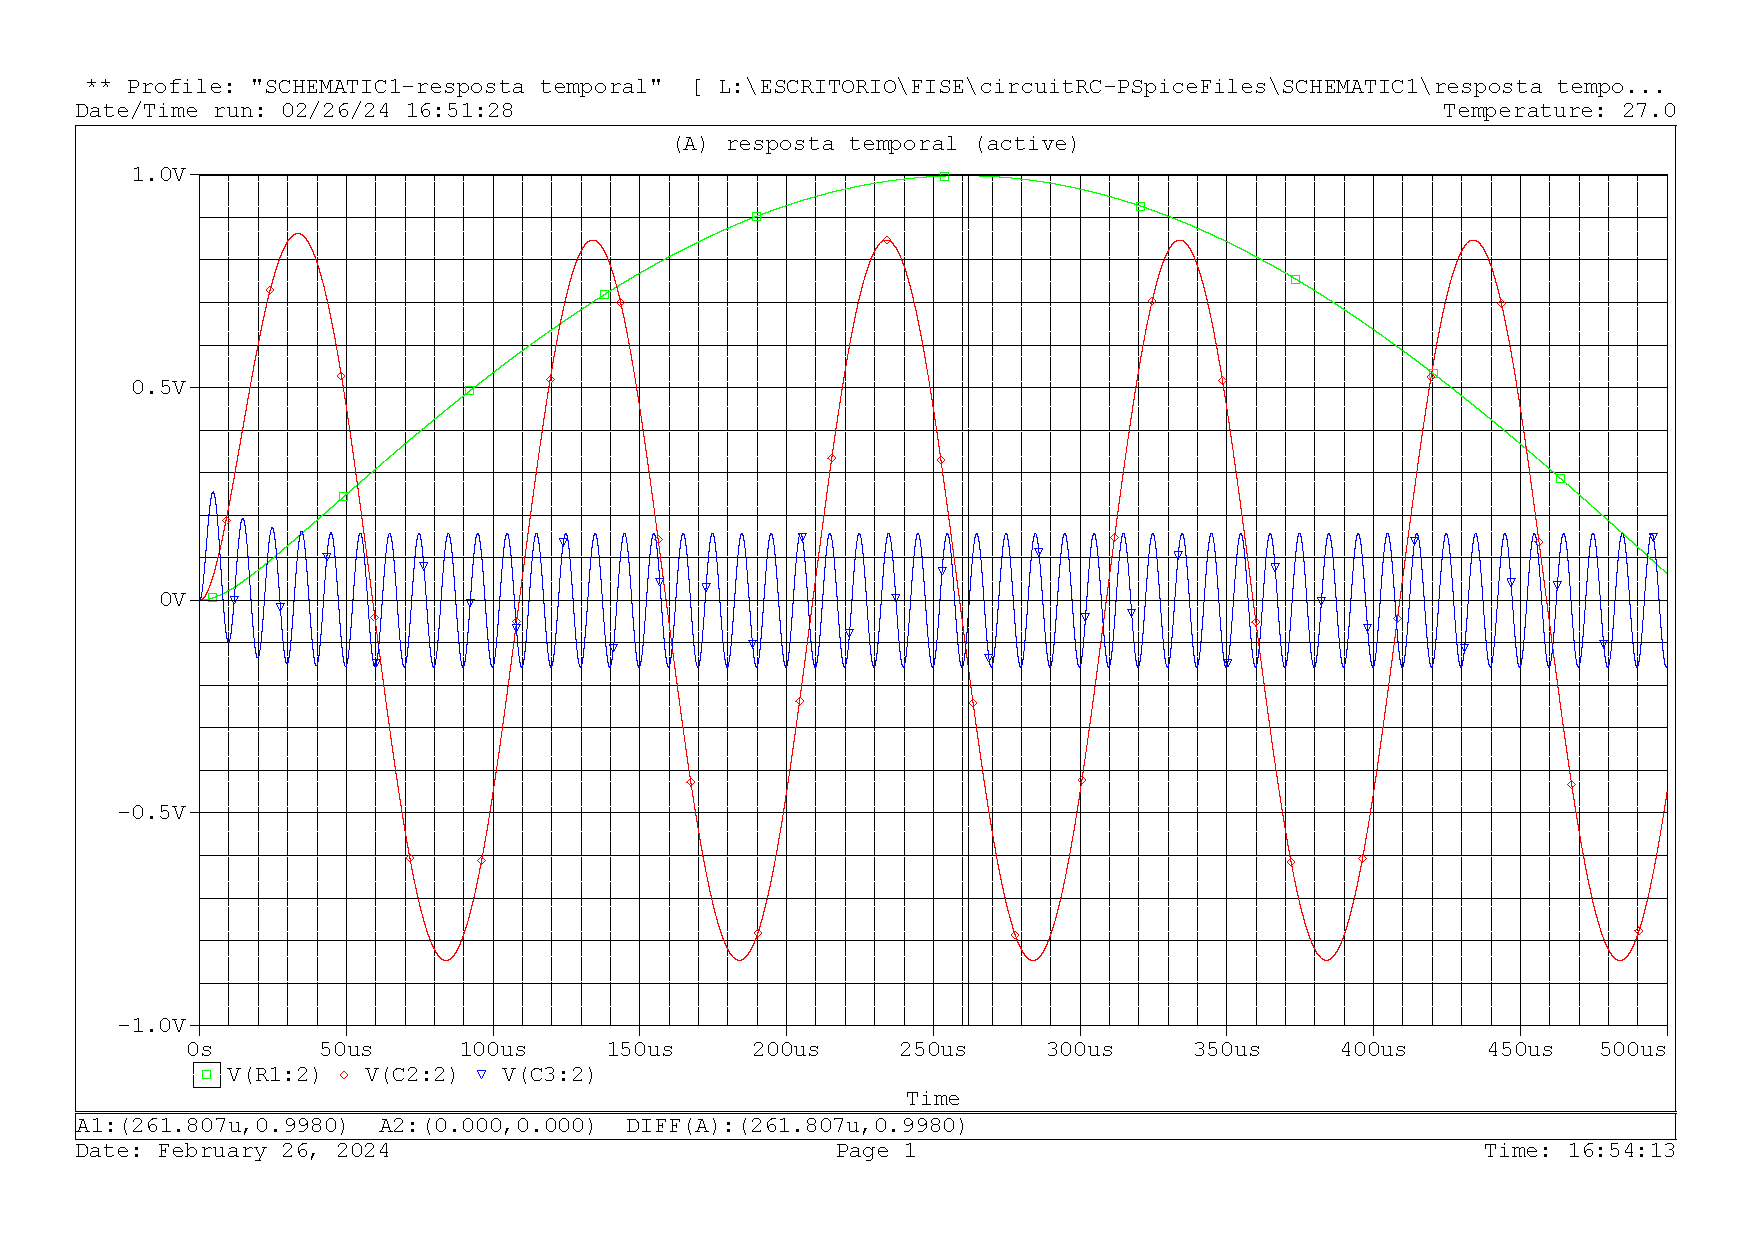
\includegraphics[width=450px]{q1.pdf}
    \caption{Les tres sortides dels tres filtres respectius passa-baixes}
    \label{fig:q1}
  \end{center}
\end{figure*}

\newthought{Qüestió 2:} La freqüència de tall és $\simeq \qty{16}{\kilo\hertz}$. Veure la figura \ref{fig:q2}. És consistent amb l'estudi previ.

\begin{figure*}
  \begin{center}
    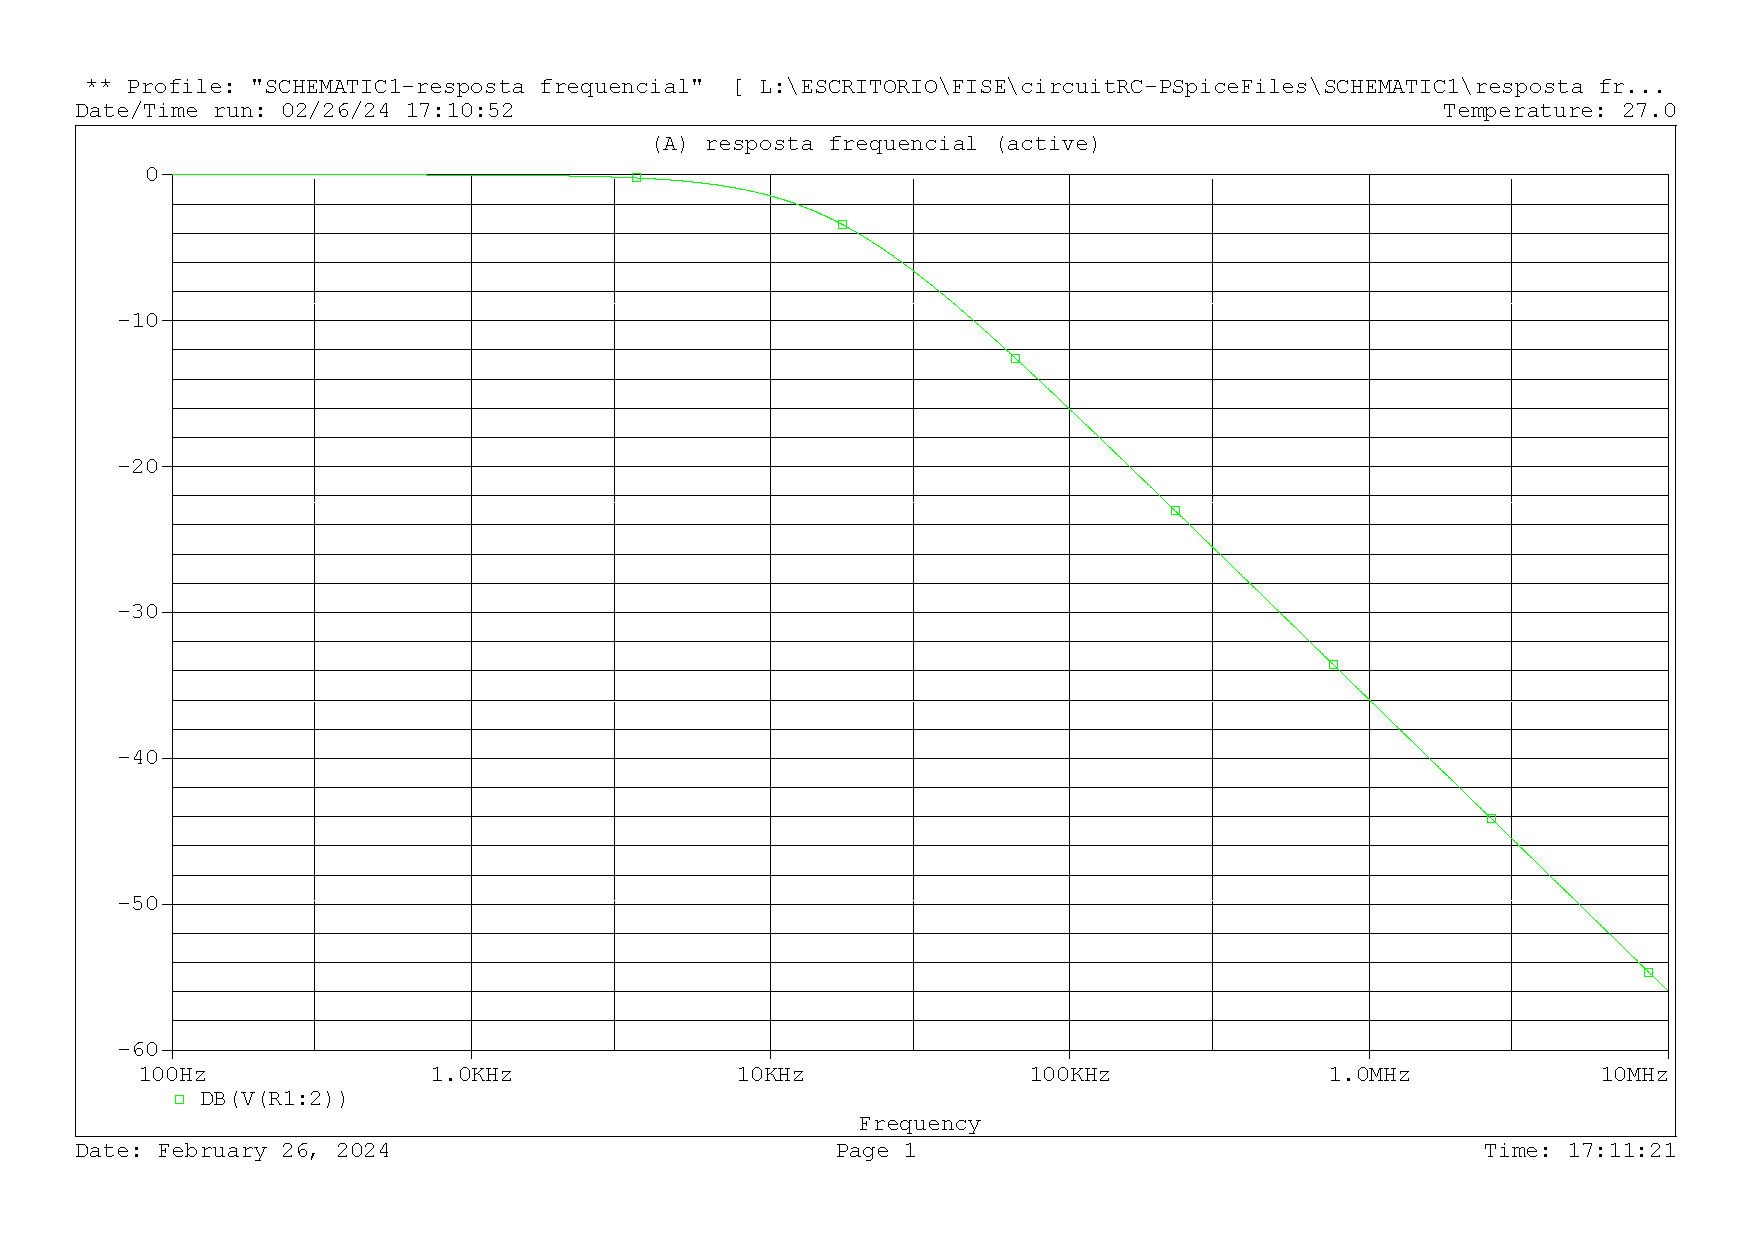
\includegraphics[width=450px]{q2.pdf}
    \caption{Funció de transferència filtre passa-baix}
    \label{fig:q2}
  \end{center}
\end{figure*}

\newthought{Qüestió 3:} Veure figura \ref{fig:q3}. El condensador es carrega i descarrega segons una exponencial inversa de factor RC. D'altra banda també es pot pensar que els primers harmònics (els més importants) pasen sense ser atenuats i els harmònics més alts no. El resultat és una petita distorsió.

\begin{figure*}
  \begin{center}
    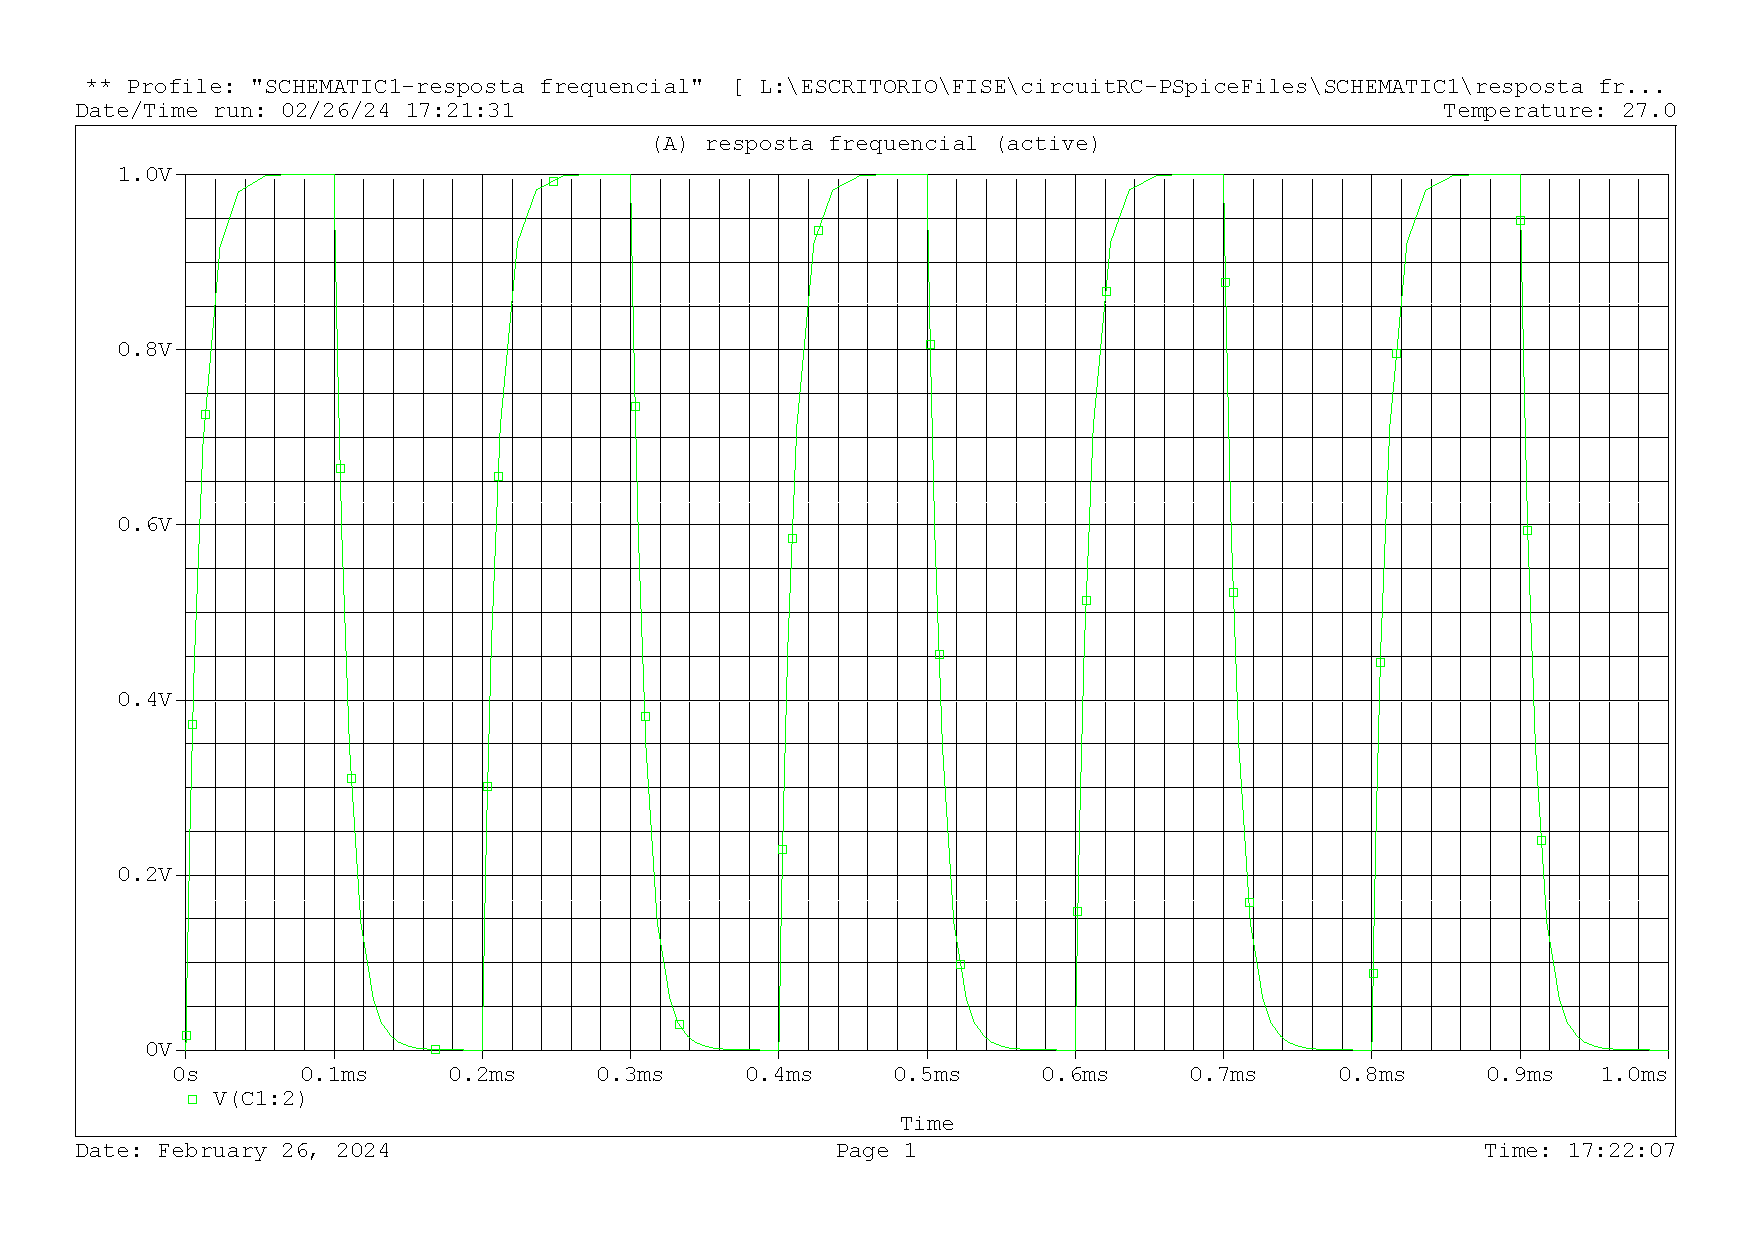
\includegraphics[width=450px]{q3.pdf}
    \caption{Resposta d'un circuit RC amb excitació pols cuadrat}
    \label{fig:q3}
  \end{center}
\end{figure*}

\newpage

\newthought{Qüestió 4:} Les amplituds es poden veure a la taula \ref{tab:t2} i a la figura \ref{fig:q4}. El pols cuadrat s'atenua completament. La freqüència de tall no ha cambiat és $\simeq\qty{16}{\kilo\hertz}$, veure la figura \ref{fig:q5}.

\begin{table}
  \begin{center}
    \begin{tabular}{@{}rccc@{}}
      \toprule
      Freqüència & \qty{1}{\kilo\hertz} & \qty{10}{\kilo\hertz} & \qty{100}{\kilo\hertz} \\
      \midrule
      Amplitud & $\simeq\qty{0}{\volt}$ & \qty{532}{\milli\volt} & \qty{950}{\milli\volt} \\
      \bottomrule
    \end{tabular}
  \end{center}
  \caption{Amplituds per freqüència}
  \label{tab:t2}
\end{table}

\begin{figure*}
  \begin{center}
    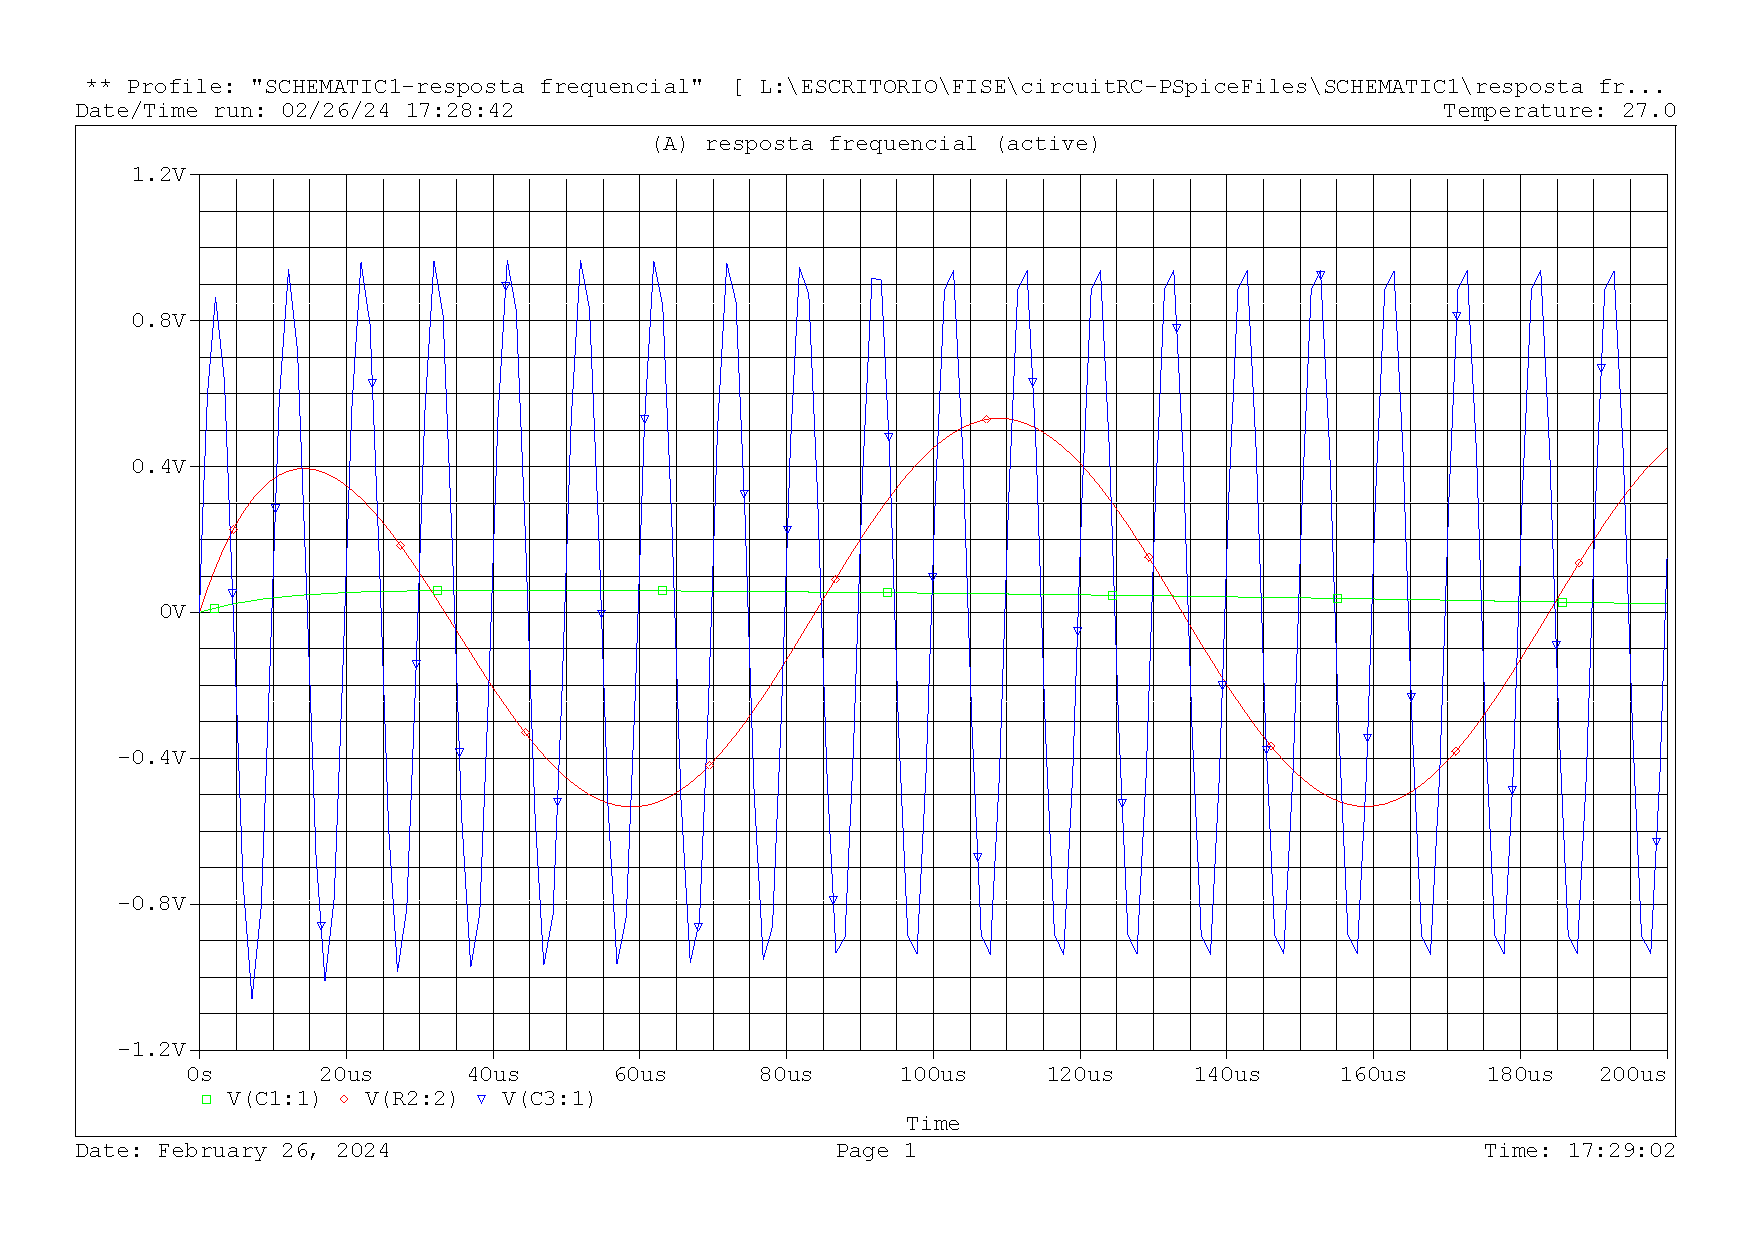
\includegraphics[width=450px]{q4.pdf}
    \caption{Les tres sortides dels tres filtres respectius passa-altes}
    \label{fig:q4}
  \end{center}
\end{figure*}

\newpage

\begin{figure*}[h!]
  \begin{center}
    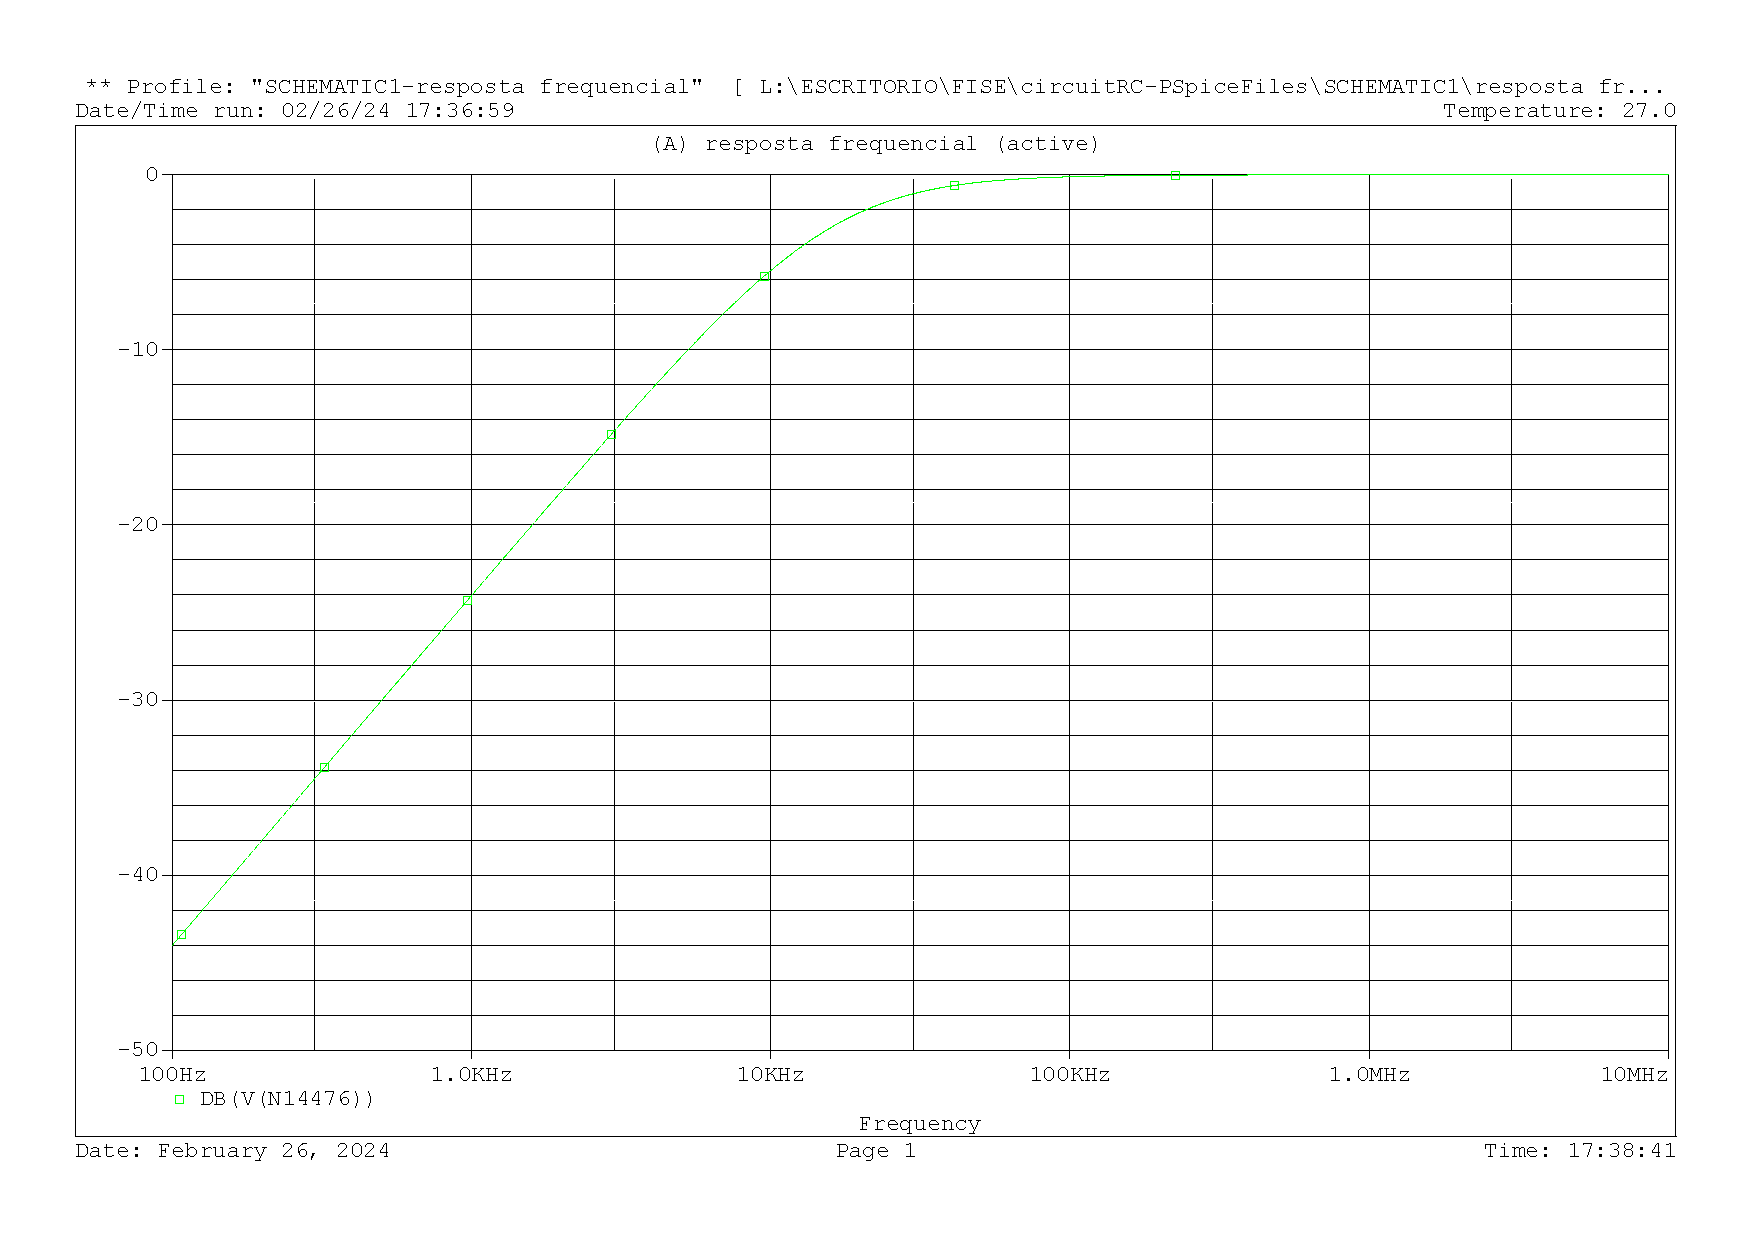
\includegraphics[width=450px]{q5.pdf}
    \caption{Funció de transferència de filtre passa-altes}
    \label{fig:q5}
  \end{center}
\end{figure*}

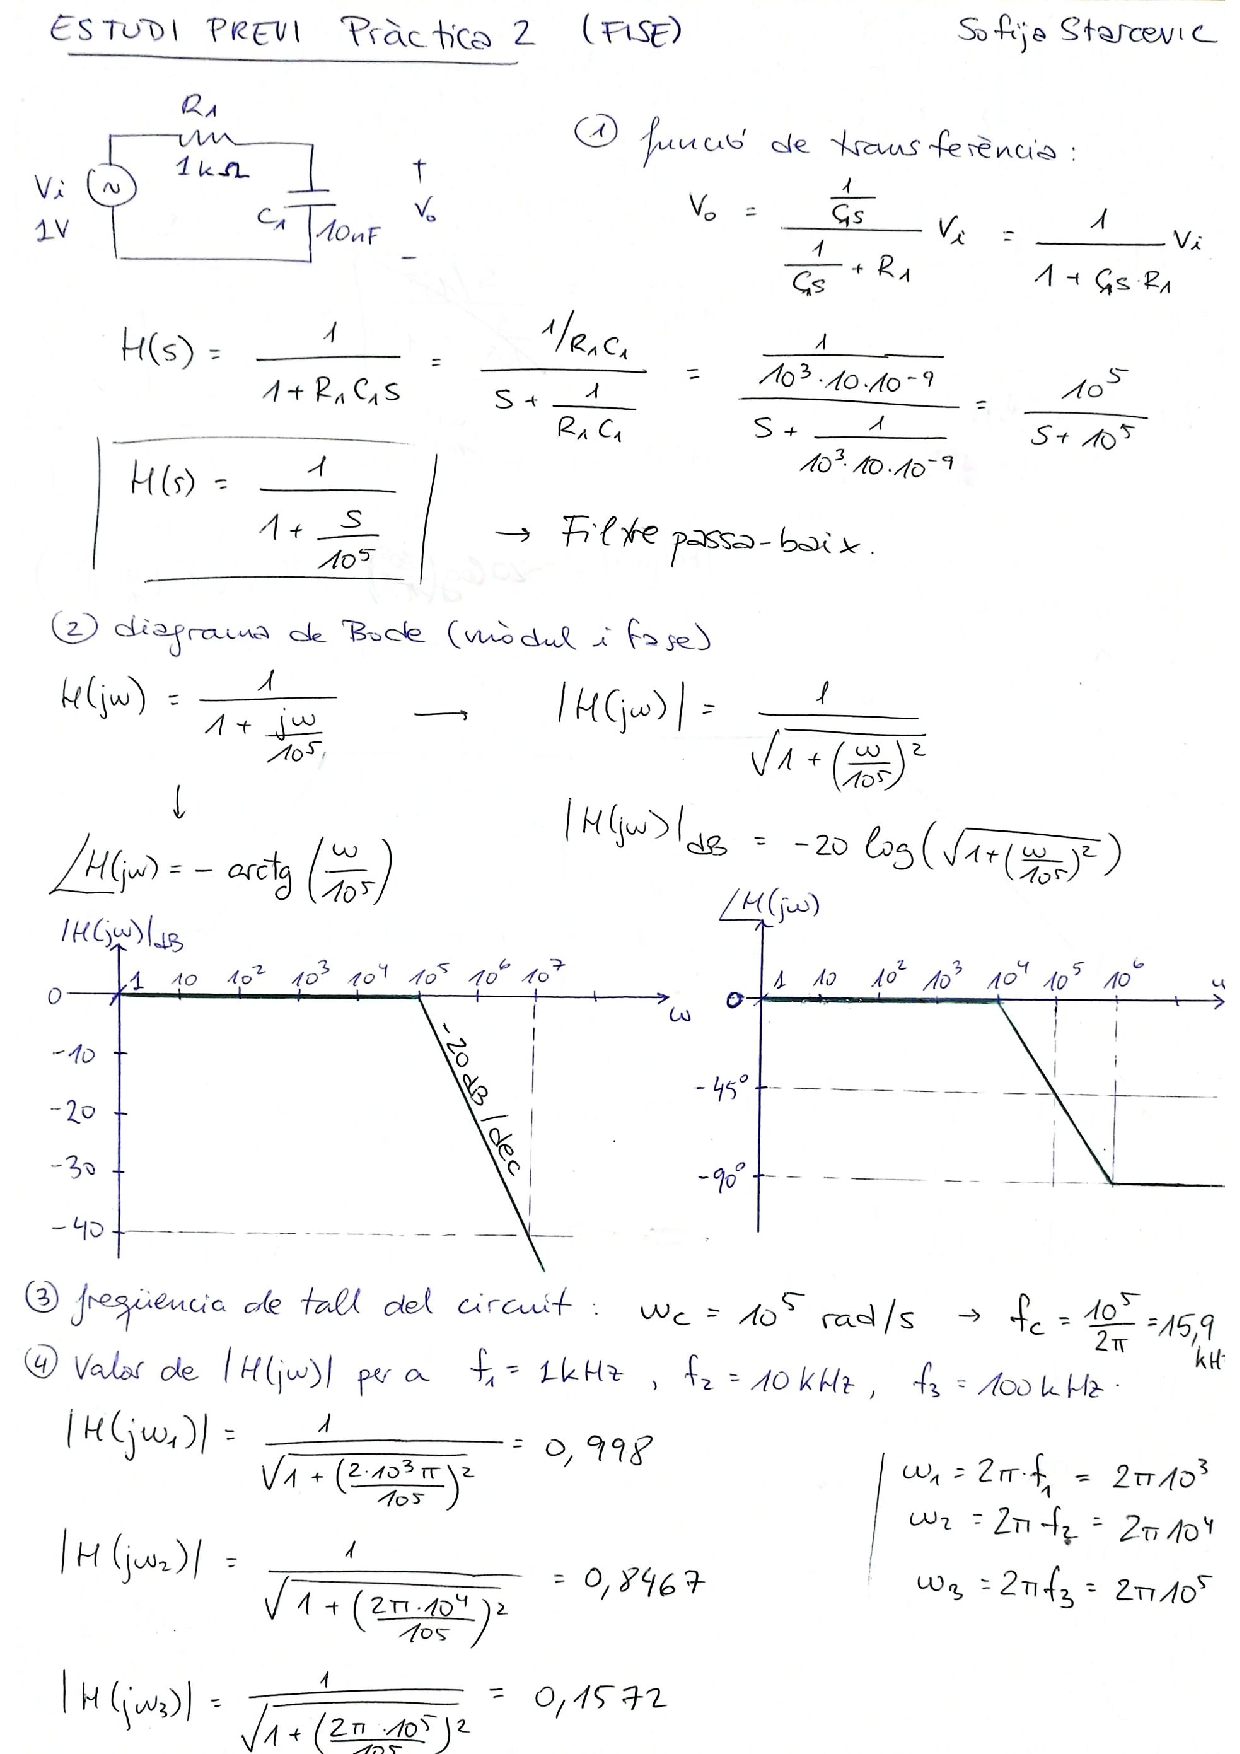
\includepdf[pages={1}]{previ1.pdf}
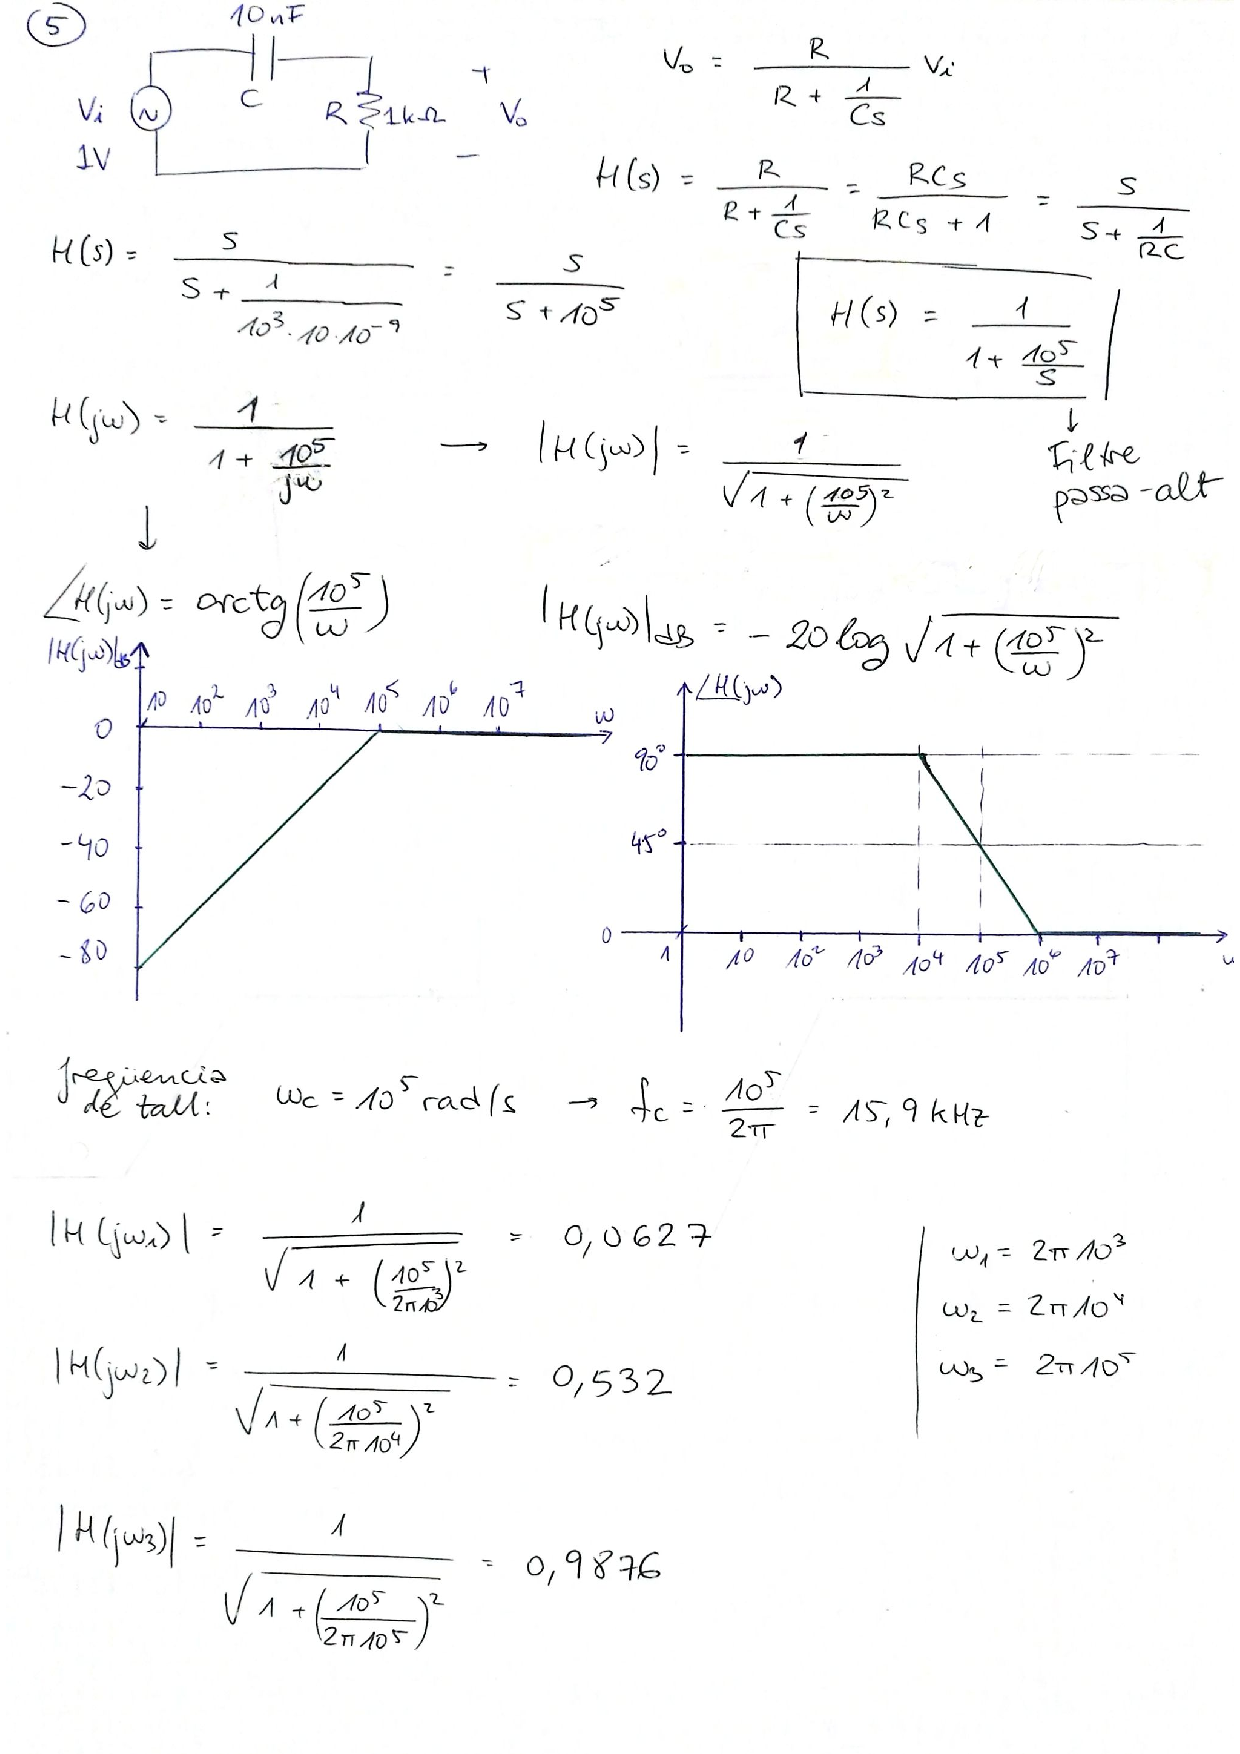
\includepdf[pages={1}]{previ2.pdf}

\end{document}